%! Author = itgramic
%! Date = 05.12.23

% Preamble
\clearpage
\subsubsection{CAP-Theorem}
Das CAP-Theorem besagt, das nur zwei der drei folgenden drei Merkmale von verteilten Systeme gewährleistet werden können\cite{EE6EQHU2}.
\begin{flushleft}
\textbf{Konsistenz - Consistency}\\
    Die Datenbank ist konsistent, alle Clients sehen gleichzeitig die gleichen Daten unabhängig, auf welchem Node zugegriffen wird.
    Hierzu muss eine Replikation der Daten an alle Nodes stattfinden und der Commit zurückgegeben werden, also eine synchrone Replikation stattfinden.
\end{flushleft}
\begin{flushleft}
\textbf{Verfügbarkeit - Availability}\\
    Jeder Client, der eine Anfrage sendet, muss auch eine Antwort erhalten.
    Unabhängig davon, wie viele Nodes im Cluster noch aktiv ist.
\end{flushleft}
\begin{flushleft}
\textbf{Ausfalltoleranz / Partitionstoleranz - Partition tolerance}\\
    Der Cluster muss auch dann noch funktionsfähig bleiben, wenn es eine beliebige Anzahl von Verbindungsunterbrüchen oder anderen Netzwerkproblemen zwischen den Nodes gibt.
\end{flushleft}
\begin{flushleft}
    Das CAP-Theorem lässt sich am einfachsten mit folgenden Venn-Diagramm visualisieren:
    \begin{figure}[H]
        \centering
        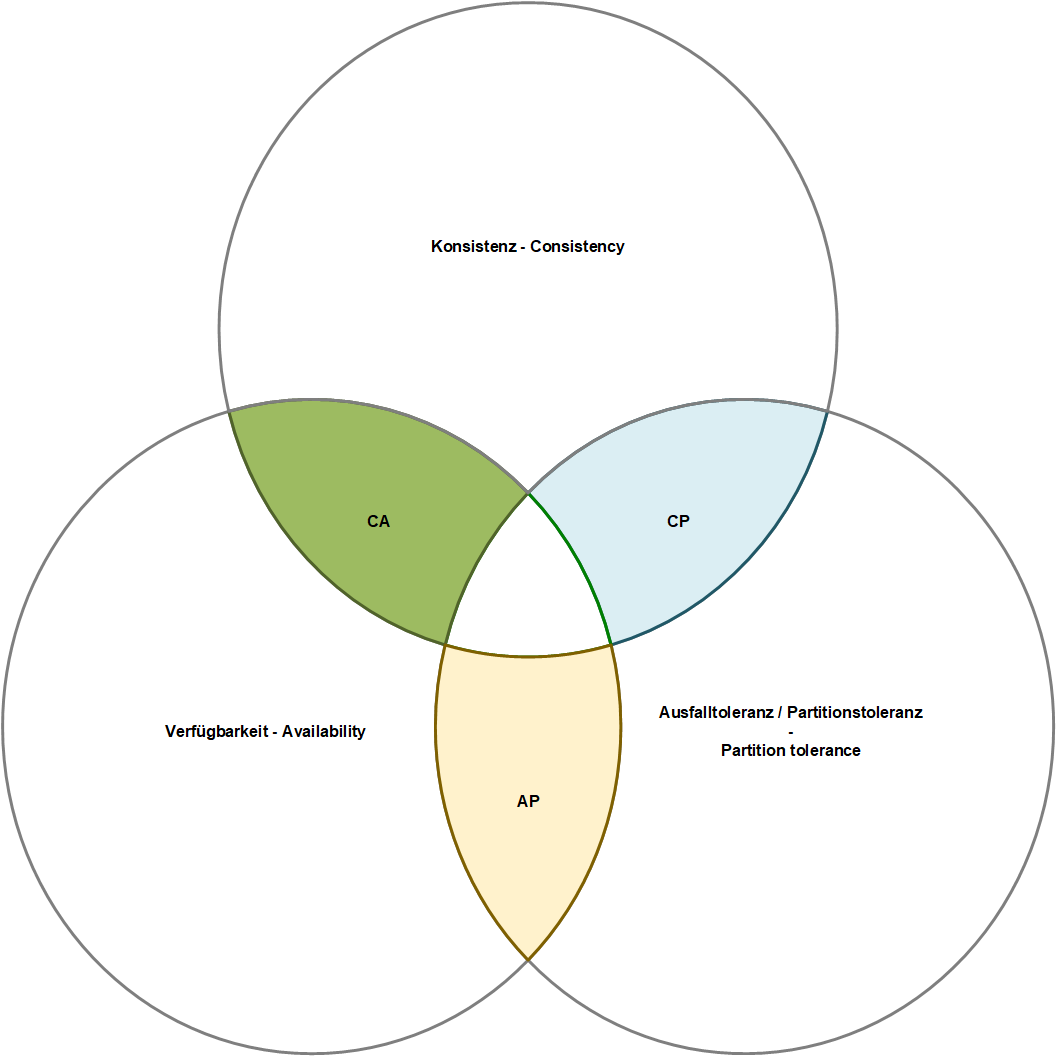
\includegraphics[width=0.5\linewidth]{source/implementation/evaluation/excursus_architecture/cap_theorem}
        \caption{CAP-Theorem}
        \label{fig:cap_theorem}
    \end{figure}
    \Gls{PostgreSQL}, \Gls{Oracle Database} oder \Gls{IBM DB2} präferieren CA, also Konsistenz und Verfügbarkeit.\\
    In dieser Diplomarbeit ist CA somit die Massgabe.
\end{flushleft}